\chapter{Obtaining Glaze Materials}
%-------------------------------------------------------------------------------
\section{Materials Suppliers}
In countries with large ceramics industries, there are suppliers that 
specialize in collecting and distributing raw materials. These may be mining 
companies that can supply specific items like clay and feldspar. If these can 
be obtained directly, it saves the costs of middlemen. However, these companies 
often deal only in large quantities. For the small producer, it is often best 
to get supplies from reliable distributors.
%-------------------------------------------------------------------------------
\subsection{Local Suppliers of Chemicals}
General chemical suppliers or pharmacies often have many of the necessary 
ingredients for glazes (which are often used in other industries). They are 
useful for obtaining small amounts of chemicals, but often their prices are 
high.
%-------------------------------------------------------------------------------
\subsection{Suppliers of Other Industries}
Glaze materials are often available from other types of suppliers. For example, 
agricultural suppliers can provide calcined limestone. Paint industries use 
materials such as iron oxide and opacifiers.
%-------------------------------------------------------------------------------
\subsection{Imported Materials}
Imported materials should only be considered if there are no local sources, as 
they are expensive and often customs and import regulations make it difficult 
or impossible for the small producer to obtain them. On the other hand, it is 
often worth paying the additional price, if it makes possible production of 
special glazes or decoration effects that are in demand in the market.

In Thailand, for example, where there is a large export market for decorative 
ceramics, many producers import clay, glazes and overglazes from Japan. Their 
profit comes from cheap labor and high value added.
%-------------------------------------------------------------------------------
\section{Materials from Natural Sources}
Small producers can mine their own materials if these are available in the 
area. Historically, pottery centers located themselves where the necessary clay 
and glaze materials were available. Where stoneware clay and high temperatures 
are used, it is possible to make glazes from low-temperature clay alone. 
Generally, stoneware glazes are made from the basic ingredients of feldspar, 
quartz, limestone and clay, which are quite common. Wood ash is another common 
base for high temperature glazes. The process of mining, selecting and grinding 
is quite time-consuming, and with the advent of modern transportation it is 
often cheaper to purchase materials from suppliers.

In Nepal, we developed low-temperature glazes based on borax, which must be 
imported. The bulk of the glaze is composed of local materials such as rice 
husk ash (for silica), limestone and local clay, which are all easy to get and 
cheap.
%-------------------------------------------------------------------------------
\subsection{Crystal Rocks}
%-------------------------------------------------------------------------------
\subsubsection{Igneous Rocks}
When the young earth slowly started to cool, different minerals formed crystals 
in the mass of molten rocks (magma). A variety of crystalline rocks were formed 
differing in composition according to their locality. For example, the igneous 
rock called basalt was created at a great depth and contains little feldspar 
compared to granite, which formed near the surface.

If rock cools very slowly, crystals have time to grow large, whereas rapid 
cooling produces small crystals. This process is still going on today where 
movement in the crust of the earth causes deep layers of molten materials to 
rise to the surface. An erupting volcano lets out hot magma, which cools 
quickly. The resulting volcanic rocks have microscopic-size crystals, since the 
rapid cooling allows little time for crystals to grow.

The most common crystal rocks used in glazes are feldspar and quartz. If a 
piece of granite is picked up and broken in two, the fresh faces of the stone 
will show a shiny surface and the crystals of the different minerals can be 
identified. The black crystals are mica or tourmaline. The yellow, white or red 
colored crystals with a pearly shine are different types of feldspar. The clear 
colorless crystals are quartz. The weathered surface of the granite will most 
probably show a rough surface with many holes, where the soluble feldspar 
crystals have been washed away by rain, whereas the less soluble crystals of 
mica and quartz remain. Coarse granite (known as pegmatite) often breaks up in 
weathering, leaving large pieces of quartz and feldspar lying on the ground. 
These can be collected, ground and used in glazes.
%-------------------------------------------------------------------------------
\subsubsection{Volcanic Rocks}
These are rocks formed by the action of volcanoes, often in the form of molten 
lava that flows out of the volcano. The crystals in the rock are extremely 
small because the lava cooled very fast. Lava is essentially a glaze and can be 
used as the basis of high temperature glazes.
%-------------------------------------------------------------------------------
\subsection{Sedimentary Rocks}
Sedimentary rocks are made of materials produced by the crumbling of old rocks. 
All rocks eventually break up in the course of time when exposed to weather, 
and the broken-up rock particles are carried away by water. These particles of 
clay and sand are transported to lower lying areas or to the sea where they 
settle one layer upon the other. In the span of millions of years, the growing 
weight of sediments causes the deeper layers to compact and gradually turn into 
rocks, called sedimentary rocks. Much later, the movement of landmasses 
sometimes turns the whole area upside down, so that the old sea floor, with its 
sedimentary rocks, becomes a new range of mountains.

The upper part of new mountains consists of sedimentary rocks resting on deeply 
set igneous rocks. Sedimentary rocks like sandstone, shale and slate can often 
be recognized by their layered structure. Limestone is a sedimentary rock 
created by the skeletons of billions of small animals that lived in the ancient 
seas. Gypsum is formed by chemical sedimentation in areas where seawater 
evaporates on a large scale. This produces a high concentration of gypsum which 
forms crystals like the formation of salt crystals in a glass of salty water.

For the glazemaker, sedimentary shale can be a source of glaze. At high 
temperatures, shale melts and with a few additions will produce glazes that are 
usually brown. Although shale often does not slake in water, it can be ground 
in a pan mill and used in glaze.
%-------------------------------------------------------------------------------
\begin{figure}[htbp!]
  \centering
  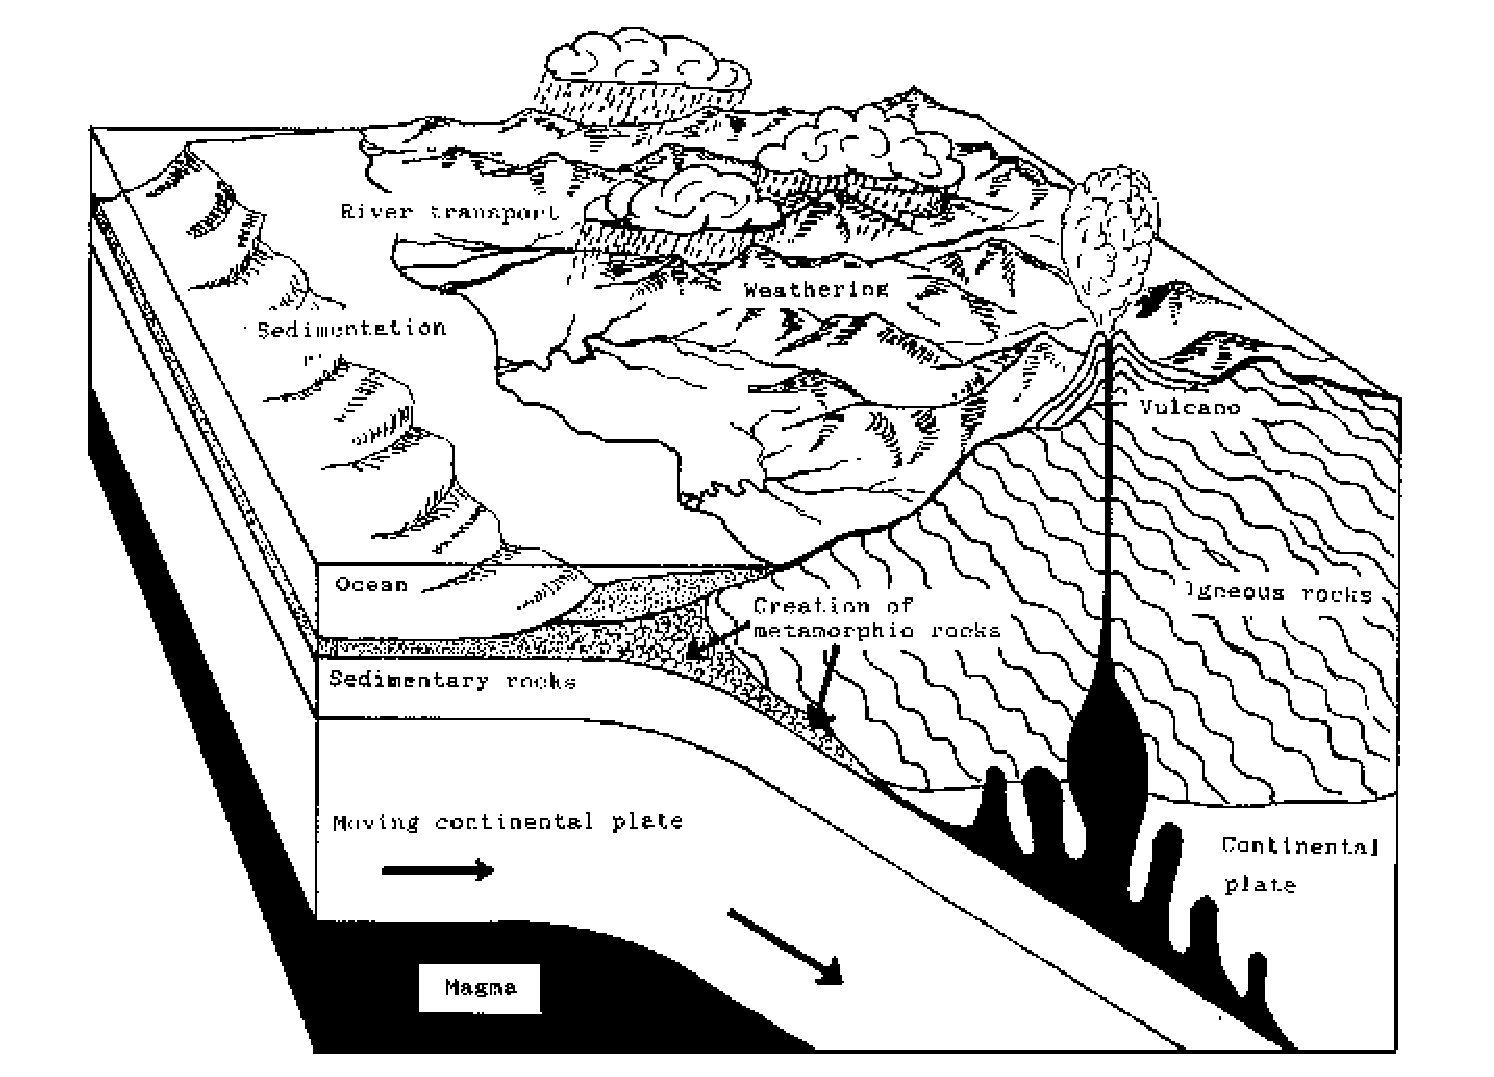
\includegraphics[width=0.9\linewidth]{img/continentalplate.eps}
  \caption{A cutout of a section of the crust of the earth shows a continental 
  plate moving under another. The friction of the plates generates heat, which 
  melts rocks and feeds a volcano. Rain falls and old rocks are weathered and 
  washed to the sea creating new layers of sediments. Later the sediments are 
  compressed into rocks.}
  \label{fig:continentalplate}
\end{figure}
%-------------------------------------------------------------------------------%-------------------------------------------------------------------------------
\subsection{Metamorphic Rocks}
Igneous and sedimentary rocks are sometimes changed into new forms by high 
temperature and pressure. Marble is an example of a metamorphic rock formed 
from the sedimentary rock limestone.
%-------------------------------------------------------------------------------%-------------------------------------------------------------------------------
\subsection{How to Get Information}
\subsubsection{Local Authorities}
First of all, information about the geology and the minerals of the region 
should be gathered from local authorities, like industrial development 
organizations, agricultural institutions, National Geological Institutes or 
mining corporations. They may have little information and the authorities may 
even say that no materials are available in the region. However, that is often 
not true and should not keep anybody from looking on his own.
%-------------------------------------------------------------------------------%-------------------------------------------------------------------------------
\subsubsection{Practical People}
It is worth talking to people who make water wells, and builders of dams and 
roads. They sometimes have useful information about the minerals of the region. 
Farmers in the area will know about the upper layers of soil on their fields 
and about local rocks. Sometimes glaze minerals are used for other purposes, 
like whitewashing houses or medicine.

The best source of information is often other potters.
%-------------------------------------------------------------------------------%-------------------------------------------------------------------------------
\subsection{Looking for Minerals}
Good places to look for minerals are in riverbeds, where many different types 
of rocks will wash down from the mountains above. Although most of these may 
not be useful, it is often possible to find quartz and feldspar. Any rock with 
an unusual color is worth testing. Rocks that are unusually heavy may contain 
metallic oxides. For the potter, however, there are few rocks that are directly 
useful, other than quartz, feldspar and limestone, and some of the volcanic 
rocks.

Other minerals that are useful in glazes are sodium and potassium compounds, 
which sometimes form on the edge of lakes, particularly in desert areas. These 
usually look like a white powder and are soluble in water.
%-------------------------------------------------------------------------------%-------------------------------------------------------------------------------
\subsection{Testing}
To begin with, the most useful test is to take a small sample of the material, 
place it in a clay bowl and fire it in a regular glaze firing. This will 
indicate if it melts or not. If it melts, it certainly can be used in a glaze. 
Materials that do not melt should not be automatically rejected, as many useful 
glaze materials (such as calcium carbonate and quartz) only melt when combined 
with other materials. The simplest way to find out if they are of use is to 
make a line blend of one of your standard glazes, combined with the unknown 
material.

Rock minerals can be identified by their crystal shape, color, specific gravity 
and hardness. If you are seriously looking for rock minerals there are good 
books presenting most common minerals with color photos.

Mohs' scale of hardness is based on the hardness of 10 different minerals. 
Window glass and a penknife are about 5.5 and a metal file about 6.5.

Two materials have the same hardness if they cannot scratch each other. Quartz 
can scratch feldspar but not topaz. In the field a piece of glass and a 
penknife are used to find out if the hardness of a rock is higher or lower than 
5.5.

If a testing laboratory is available, samples can be sent there for chemical 
analysis. This is usually expensive but may be helpful if the material looks 
useful after firing.
%------------------------------------------------------------------------------
\begin{center}
        \renewcommand{\arraystretch}{1.5}
          \begin{table}\centering
    \begin{tabular}{|c|c|}\hline
      \textbf{Mineral}&\textbf{Hardness}\\\hline\hline
      %------------------------------------------------------------------------------
      Talc&1\\\hline
      %------------------------------------------------------------------------------
      Gypsum&2\\\hline
      %------------------------------------------------------------------------------
      Calcite&3\\\hline
      %------------------------------------------------------------------------------
      Fluorspar&4\\\hline
      %------------------------------------------------------------------------------
      Apatite&5\\\hline
      %------------------------------------------------------------------------------
      Orthoclase feldspar&6\\\hline
      %------------------------------------------------------------------------------
      Quartz&7\\\hline
      %------------------------------------------------------------------------------
      Topaz&8\\\hline
      %------------------------------------------------------------------------------
      Corundum&9\\\hline
      %------------------------------------------------------------------------------
      Diamond&10\\\hline
    \end{tabular}
    \caption{Mohs' Scale of Hardness.}
    \label{tab:mohs}
  \end{table}
\end{center}
%------------------------------------------------------------------------------
\section{Other Sources of Materials}
Recycled materials are often useful in glazes. These may be by-products from 
other industries, such as rice husk ash or bone meal, or waste materials. Some 
other sources of useful materials are discussed below.
%------------------------------------------------------------------------------
\subsection{Metallic Oxides}
Metallic oxides are used as coloring agents in glazes. Commonly available are:

Iron oxide, which can be obtained by scraping rust from old steel. It is often 
possible to get this from paint and hardware suppliers, who use "red oxide" for 
coloring paint and cement.

Manganese dioxide, which is the main ingredient in torch batteries (the black 
substance which can be removed from old batteries).

Copper oxide, which can be collected from makers of copper pots. The oxide is 
the black powder that forms on the surface of copper when it is heated. Another 
way is to fire copper wire in the kiln and to use the resulting black copper 
oxide.
%------------------------------------------------------------------------------
\subsection{Ashes}
Wood ashes are used as the basis for high temperature glazes, since they 
contain sodium, potassium, silica and other ingredients. Early glazes were 
often simple mixtures of wood ash and clay. Most wood ash is suitable for this 
purpose, but each type of wood will produce different characteristics and will 
have a different melting point. So it is important to have a consistent supply. 
Ash must be sieved to remove unburned material and is usually washed in water 
and dried before use. If it is not washed it contains more fluxes but they are 
soluble and make the glaze slip caustic.

At cone 8 to 11, a good starting point is 2 parts ash, 2 parts feldspar and 1 
part clay. Ash glazes have general limits as shown in 
table~\ref{tab:limits}.

Rice husk ash contains more than 90\% silica, so it can be used instead of 
quartz in many cases. For accuracy, it should be burned white--if there is 
much black carbon in it, it will make calculations incorrect. 

In Appendix~\ref{sec:appendix_composition} the chemical composition of 
different ashes is given.
%------------------------------------------------------------------------------
\begin{center}
        \renewcommand{\arraystretch}{1.5}
          \begin{table}\centering
    \begin{tabular}{|c|c|}\hline
      \textbf{Material}&\textbf{Percent}\\\hline\hline
      %------------------------------------------------------------------------------
      Ash&20--70\%\\\hline
      %------------------------------------------------------------------------------
      Feldspar&20--70\%\\\hline
      %------------------------------------------------------------------------------
      Whiting&5--20\%\\\hline
      %------------------------------------------------------------------------------
      Flint&15--25\%\\\hline
      %------------------------------------------------------------------------------
      Clay&5--20\%\\\hline
    \end{tabular}
    \caption{Limits of material content in glazes.}
    \label{tab:limits}
  \end{table}
\end{center}
%------------------------------------------------------------------------------
\section{Storing, Packaging, and Labeling}
If you use local materials, they will change from time to time. For this 
reason, it is best to store as much material as possible and to check each new 
batch by trying it in a standard glaze. For example, feldspar tends to be 
variable and, as the mine is used, the chemical composition will change. 
Suppliers of feldspar usually keep several large storage areas of material from 
different parts of the mine. In order to keep it uniform, they mix the 
different feldspars together when supplying.

Some materials are damaged by water. Borax, boric acid, soda ash and plaster of 
parts should all be kept in a dry place. In particular, soda ash absorbs water 
(up to 7\% after one year, 11\% after two years) and will thereafter no longer 
be effective as a slip deflocculant; and plaster will not set correctly after 
damp storage.

When you get local materials, each batch should be kept separately and labeled 
with date and source. It is often a good idea to purchase more material when 
your old supply is about 50\% finished and to test it to see if it is the same 
or not. If it is not greatly different, the new material can be mixed with the 
old and your glaze will not change unexpectedly.

A good labeling system is very important, as most glaze chemicals look rather 
alike. Never depend on your memory - keep a permanent label on the bag or jar 
of material. Additionally, if you order bags of material from a supplier, ask 
him to label the outside of the bag, and also to put a label inside the bag as 
labels are often lost in shipping.
%------------------------------------------------------------------------------